\documentclass[tikz]{standalone}

\begin{document}

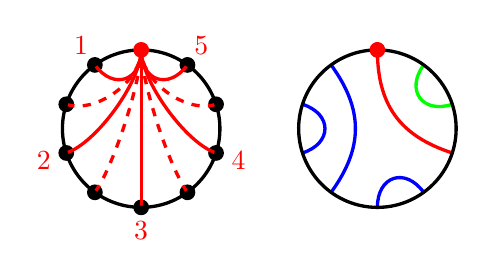
\begin{tikzpicture}[very thick]

    \foreach \i in {1, 2, ..., 9} {
    \fill ({90+\i*360/10}:1) circle (.1);
    }
    \foreach \i in {1, 2, ..., 5} {
        \draw[red] ({54+2 * \i*360/10}:1) .. controls +({54+2*\i*360/10}:-.4) and +(0, -.4) .. (90:1);
        \draw[red] ({54+2 * \i*360/10}:1.3) node{\i};
    }
    \foreach \i in {2, 4, ..., 9} {
        \draw[red, dashed] ({90+\i*360/10}:1) .. controls +({90+\i*360/10}:-.4) and +(0, -.4) .. (90:1);
    }
    \draw (0, 0) circle (1);
    \fill[red] (90:1) circle(.1);

    \begin{scope}[shift={(3, 0)}]
        \begin{scope}[rotate={3.5*360/10}]
        \begin{scope}[blue]
            \draw ({360/10}:1) .. controls ({1*360/10}:.6) and ({2*360/10}:.6) .. ({2*360/10}:1);
            \draw ({0*360/10}:1) .. controls ({0*360/10}:.3) and ({3*360/10}:.3) .. ({3*360/10}:1);
            \draw ({4*360/10}:1) .. controls ({4*360/10}:.6) and ({5*360/10}:.6) .. ({5*360/10}:1);
        \end{scope}
        \begin{scope}[green]
            \draw ({7*360/10}:1) .. controls ({7*360/10}:.6) and ({8*360/10}:.6) .. ({8*360/10}:1);
        \end{scope}
        \begin{scope}[red]
            \draw ({6*360/10}:1) .. controls ({6*360/10}:.3) and ({9*360/10}:.3) .. ({9*360/10}:1);
        \end{scope}
        \draw (0, 0) circle (1);
        \fill[red] ({9*360/10}:1) circle(.1);
    \end{scope}
    \end{scope}
\end{tikzpicture}

\end{document}
